\section{Systèmes P2P exploitables par les MMOGs distribués}
	Des systèmes pair à pair sont déjà exploitables par les MMOGs sitribuées, un tour d'horizon de ceux-ci va permettre de mettre en avant ce qu'ils apportent. Les concepts d'aire d'intérêt, de découpage de la carte et d'overlay vont être passé en revue.
	\subsection{Area Of Interest}
	Dans plusieurs articles, la notion de \textit{Area Of Interest}~\cite{1403002,1267692,1015507} va apparaître ce qui montre l'utilité de ce concept. Nous pouvons déjà retrouver ce principe sous le nom de \textit{Local Awareness} dans Sollipsis, l'idée principale de ce mécanisme est qu'une entité n'a pas besoin de connaître l'ensemble du monde virtuel à chaque instant. Alors nous allons mettre en place une zone dans laquelle l'entité sera tenue informée des différentes modifications qui seront faites sur les objets et les autres entités qui se trouvent dans la zone (voir schéma~\ref{AOI}). Si une entité modifie sa représentation virtuelle, seulement les entités qui sont dans sa zone seront directement informées.\\

	%\subsubsection{Mercury}
	\par Dans Mercury~\cite{1015507}, le concept d'Area Of Interest va pouvoir être utile avec le mécanisme de publish-subscribe qui est mis en place. Ce mécanisme de publish-subscribe permet l'abonnement et le désabonnement aux mises à jour d'un objet, et il permet donc d'envoyer un objet vers les nœuds qui sont abonnés.\\
	%\subsubsection{Colyseus}
	\par Colyseus~\cite{1267692} est un travail postérieur à Mercury, les principes sont les mêmes avec l'utilisation de \textit{range-queriable} DHT ou de DHTs pour stocker les informations. Les \textit{range-queriable} DHTs vont s'organiser en un overlay circulaire où chaque nœud adjacent est responsable d'une suite continue de clés. Grâce à cela, il sera possible de prendre les coordonnées \textit{X} comme clé et ainsi les performances seront bien meilleures qu'avec des DHTs normales (aléatoire). Les différents résultats réalisés montrent bien que les \textit{range-queriable} DHTs utilisent moins de bande passante que les DHTs normales. \\
	%\subsubsection{Donnybrook}
	\par Dans Donnybrook~\cite{1403002}, le concept d'Area Of Interest fait référence au travail réalisé dans Colyseus. Comme chaque joueur envoie ses mises à jour à chaque joueur qui se trouve dans sa zone, il faut une limitation du nombre de joueurs dans une même zone. Donnybrook introduit la notion de \textit{player's interest set}, un joueur va pouvoir se concentrer sur un nombre fixe de joueurs (cinq dans l'article), à la différence du nombre d'objet dans l'AOI qui peut varier. Un mécanisme d'abonnement sera mis en place pour s'échanger les informations entre les joueurs. Un mécanisme d'\textit{intérêt estimé} est mis en place pour définir les joueurs qui feront partis de son \textit{interest set}. Plusieurs critères sont pris en compte pour choisir les joueurs qui seront sélectionnés. Trois principales propriétés sont prises en compte: la proximité spatiale entre les joueurs, les objectifs des joueurs et les interactions récentes que les joueurs peuvent avoir eu entre les deux joueurs.\\
	\vspace{5mm}
        \begin{figure}[!h]
        \centering
        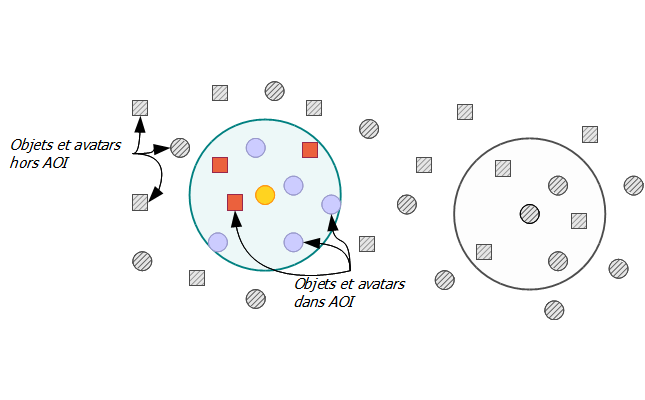
\includegraphics[scale=0.65]{./Ressources/Images/AOI.png}\\
        \caption{Principe de l'\textit{Area Of Interest}}
        \label{AOI}
        \end{figure}
	\vspace{5mm}
	\subsection{Découpage de la carte}
	Pour plusieurs raisons, dont l'équilibrage de charge, le monde a été découpé en plusieurs zones. Différentes techniques pour le découpage ont été étudiées, l'une des plus courantes est d'utiliser le découpage grâce au découpage de Voronoi~\cite{1016552}, c'est de cette technique que la triangulation de Delaunay s'inspire. Les découpages suivant ces principes sont répandus car un découpage aléatoire ne prendrait pas en compte la densité des objets dans le monde qui peut être très variable entre les régions. Le principe est de découper la monde en zone en fonction de la distance entre les différents objets qui se trouvent dans l'environnement. Dans une région, on aura un objet qui sera entouré de ses voisins. La frontière entre la région de deux voisins se trouve au milieu d'une droite séparant les deux voisins. Comme il est possible de voir sur le schéma~\ref{Voronoi}, les zones ont des formes et des tailles différentes. Nous avons ainsi des zones qui comprennent un seul nœud. La différence entre la triangulation de Delaunay et le découpage de Voronoi est que pour la première, les arrêtes seront les droites entre les sommets si ils sont voisins et dans le deuxième cas, les arrêtes seront formées grâce aux médiatrices des arrêtes de la triangulation de Delaunay.\\ 
	\vspace{5mm}
        \begin{figure}[!h]
        \centering
        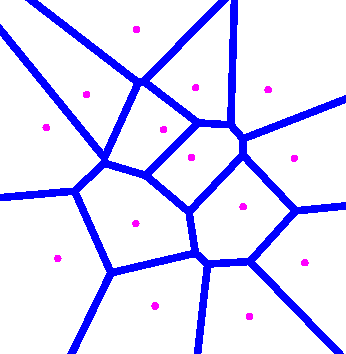
\includegraphics[scale=0.45]{./Ressources/Images/voronoi.png}\\
        \caption{Principe du découpage de Voronoi}
        \label{Voronoi}
        \end{figure}
        \vspace{5mm}

	\subsection{Overlays}
	Plusieurs travaux sur la modification de l'overlay ont été fait~\cite{999375,10.1109/SRDS.2006.33,citeulike:6040284}, le but principal de ces travaux est de mettre en place un overlay qui puisse facilement s'adapter aux besoins des nœuds. Un overlay est un réseau informatique formant un graphe au sein duquel le voisinage de chaque nœud est déterminé selon un critère logique. Dans l'architecture pair à pair, il n'y a pas de connaissance globale, il n'y a qu'une connaissance locale (voisinage). Le but est de faire des liens entre les nœuds qui sont intelligents, nous verrons des overlays avec différents degrés de prise en compte de l'application. 
		\subsubsection{Semantic overlay}
			Le but principal de cet overlay sémantique~\cite{999375} est de créer des liens entre des nœuds qui s'intéressent aux mêmes documents, car la recherche de fichiers est devenue très importante au moment de l'arrivée des logiciels de partage de fichiers tel que Napster, Gnutella, KaZaA, etc. L'approche consiste à constituer des groupes sémantiques avec les documents et de construire un overlay au dessus du réseau pour chaque groupe. Le problème est donc d'identifier et de constituer des groupes efficacement. Trois stratégies ont été mises en place:
		\begin{itemize}
		\renewcommand{\labelitemi}{$\bullet$}
                	\item \textit{LRU:} Stratégie basée sur les éléments les plus récemment utilisés
                	\item \textit{History:} On maintient les liens sémantiques vers la même classe de préférence, cette technique oblige le maintien d'un nœud \textit{counter}. C'est une technique lourde en nombre de messages et en stockage, de plus il peut y avoir des problèmes avec les \textit{counters}.
	                \item \textit{Popularity:} Création de liens entre les nœuds du même type, introduction de deux paramètres: Numrep (nombre de réponse positive pour obtenir le document) et Lastreply (date de la dernière réponse )
        	\end{itemize}
	        Les résultats montrent que Popularity est l'algorithme le plus adapté, cette stratégie a un bon compromis entre efficacité et complexité de mise en place.

		\subsubsection{Application-Malleable Overlay}
			Il y a plusieurs types d'overlay, certains ne prennent pas en compte l'application, d'autres le font seulement au démarrage, d'autres essayent de réagir aux évènements de l'application. MOve~\cite{10.1109/SRDS.2006.33} souhaite mettre en place un overlay malléable, c'est à dire que les communications de l'application distribué vont influencer la structure de l'overlay. Les deux buts principaux sont d'optimiser les performances de l'overlay et de garder les propriétés de tolérance aux fautes et de passage à l'échelle. Les auteurs mettent en place deux types de liens:
		\begin{itemize}
	        \renewcommand{\labelitemi}{$\bullet$}
	                \item \textit{Lien non-applicatif:} Ils maintiennent l'overlay global proche d'un graphe aléatoire avec un faible degré de clustering (regroupement).
        	        \item \textit{Lien applicatif:} Ils  permettent de créer un graphe fortement connecté, pour regrouper les nœuds. Chaque nœud d'un groupe crée aléatoirement des liens applicatifs vers des membres du groupe. Cela va permettre une rapide propagation des états lors des updates et des messages applicatifs multicast.
        	\end{itemize}
        Cette solution offre différentes possibilités d'ajout de nœud, de détection de défaillance, de remplacement de lien, etc. \textit{group}-based applications influencent l'overlay sous-jacent en remplaçant les liens inter nodes par des liens entres les applications. L'algorithme maintient une bonne connectivité.
		\subsubsection{Voronoi-based Overlay Network}
		 	VON veut exploiter la localité des intérêts des utilisateurs pour maintenir la topologie pair à pair avec un faible \textit{overhead}. VON utilise un principe d'AOI dynamique, il utilise le découpage de Voronoi et chaque nœud est représenté par un site dans le diagramme. VON introduit trois procédures principales :
		\begin{itemize}
	        \renewcommand{\labelitemi}{$\bullet$}
                	\item \textit{Join Procedure:} Le textit{joining node} contacte le server pour avoir un ID unique, puis envoie une requête avec ses coordonnées à tous les nœuds existants. Création de la liste des voisins, mis à jour chez les voisins, etc.
                	\item \textit{Move Procedure:} Lorsque un nœud bouge ses coordonnées sont mises à jour chez ses voisins (gestion si nœud est à la limite de la région, si il y a des nouveaux voisins, etc).
                	\item \textit{Leave Procedure:} Le nœud se déconnecte (qu'importe sa raison et la manière) et ses voisins vont se mettre à jour.
        	\end{itemize}
        	VON permet de gérer un grand nombre d'utilisateurs et de garder un topologie consistante. Il y a beaucoup de messages introduits par l'AOI et si la vitesse des utilisateurs est trop importante, on a des problèmes pour notifier les nouveaux voisins.

		

	
